\section{Agent-Based Simulations}
\label{sec:section4}  
\subsection{PREE Convergence}
Given the lack of accessible SBDP user data, I developed on agent-based simulation environment to explore the evolution of both behavioural and market-level dynamics under the above theoretical foundation. 
Agent-based modelling (ABM) is used to study how \textit{``macro phenomena emerges from micro level behaviour among a heterogeneous set of interacting agents''} \citep{janssen2005agent}, and it has been successfully applied by recent work on matching platforms \citep{immorlica2021designing} to help identify, and understand the structure of, equilibrium states, which can be computationally expensive to approximate (and in some cases even non-existent).

\begin{figure}[ht]
    \centering
    \caption{Agent-Based Simulation Convergence}
    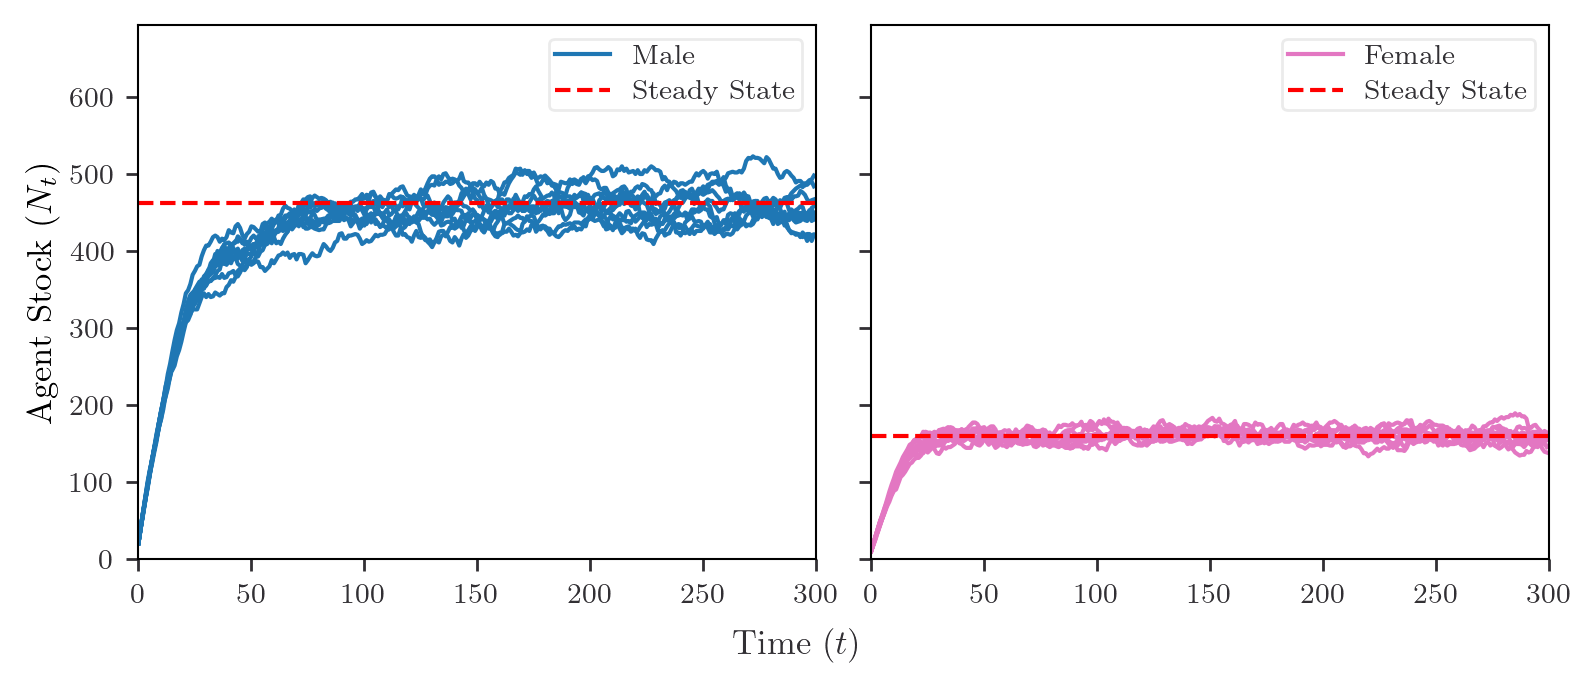
\includegraphics{abm-conv-imbalanced.png}
    \label{fig:abm-conv} 
\end{figure}

To start, I explore the convergence and stability of the SBDP market under arbitrary exogenous settings. In particular, \autoref{fig:abm-conv} shows the simulated evolution of (sex-specific) agent masses over 300 time periods, with a 2:1 ratio between male and female arrival flows. This simulation was conducted under PREE conditions; that is, with agents using optimal policies for some fixed steady state even when this is not equal to the current platform state.  
As evident from these results, this process converges onto the fixed steady state computed using the procedures in \autoref{sec:section3.1}. Furthermore, the ABM simulations show that the long side of the market (males) takes considerably longer to converge onto its steady-state level. One technical point worth noting is that the above simulations depict \textit{agent stocks} as opposed to \textit{agent masses}, as per our continuum model. Thus, because agent departures and pairings follow random processes, the above equilibrium acts as a \textit{stochastic steady state}, with convergence occurring in the stationary sense rather than in typical deterministic fashion. Nevertheless, I examine the limiting case of these dynamics, with \autoref{fig:abm-conv-ssize} depicting how, by the law of large numbers, stationary deviations around the steady state level become negligible as the agent stocks tend to infinity. 

\begin{figure}[ht] 
    \centering
    \caption{Agent-Based Simulation Convergence with Varying Sample Sizes}
    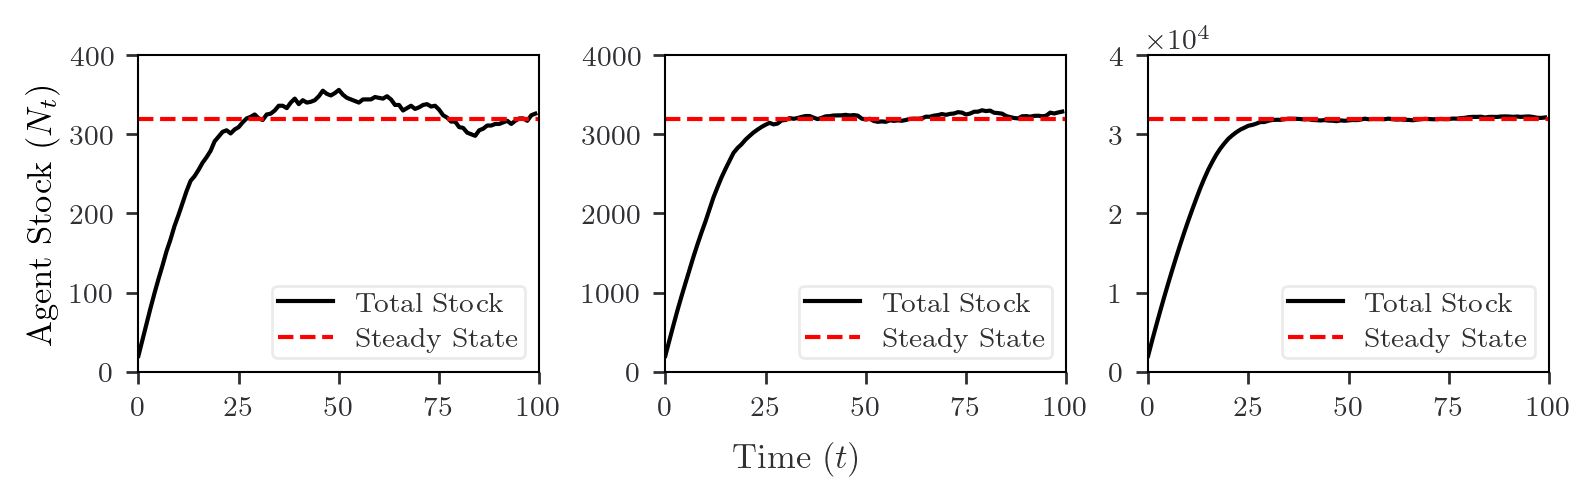
\includegraphics{abm-conv-ssize.png}
    \label{fig:abm-conv-ssize}
\end{figure} 

\subsection{Myopic Best-Response Dynamics}
Finally, I simulate the SBDP market under myopic best-response dynamics to explore whether if steady state equilibria can be reached using a more robust process of gameplay. For this simulation, agents re-compute their optimal policies at the start of every time period given the current market state, unlike with PREE simulations where optimal policies are computed once with respect to the SSE for some given exogenous settings. This process is \textit{myopic} in the sense that optimal policies are computed accounting only for the current state but not for its dynamic evolution; yet it is still more robust than PREE as constant feedback between policies and states could create outward-spiralling dynamics that prevents convergence onto SSE. The results of these simulations over 120 time periods are presented in \autoref{fig:abm-br-balanced}, showing that, both in the case of balanced and unbalanced markets, the SSE can be attained using myopic best response dynamics.

\begin{figure}[ht] 
    \centering
    \caption{Agent-Based Simulation Under Myopic Best Response Dynamics}
    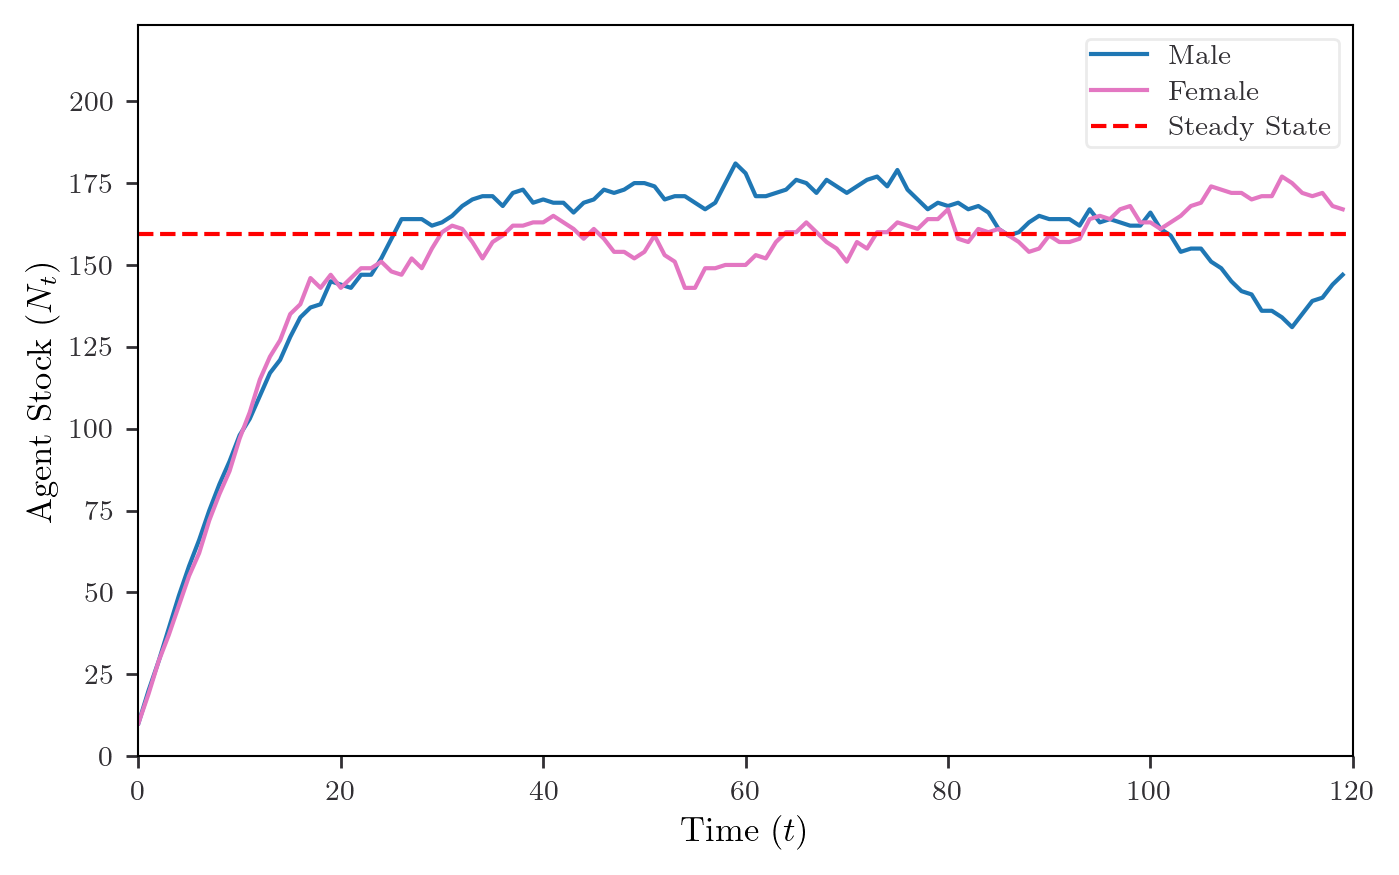
\includegraphics{abm-br-balanced.png}
    \label{fig:abm-br-balanced}
\end{figure}  


